\documentclass{standalone}
\usepackage{tikz}
\usetikzlibrary{patterns, positioning}

\begin{document}
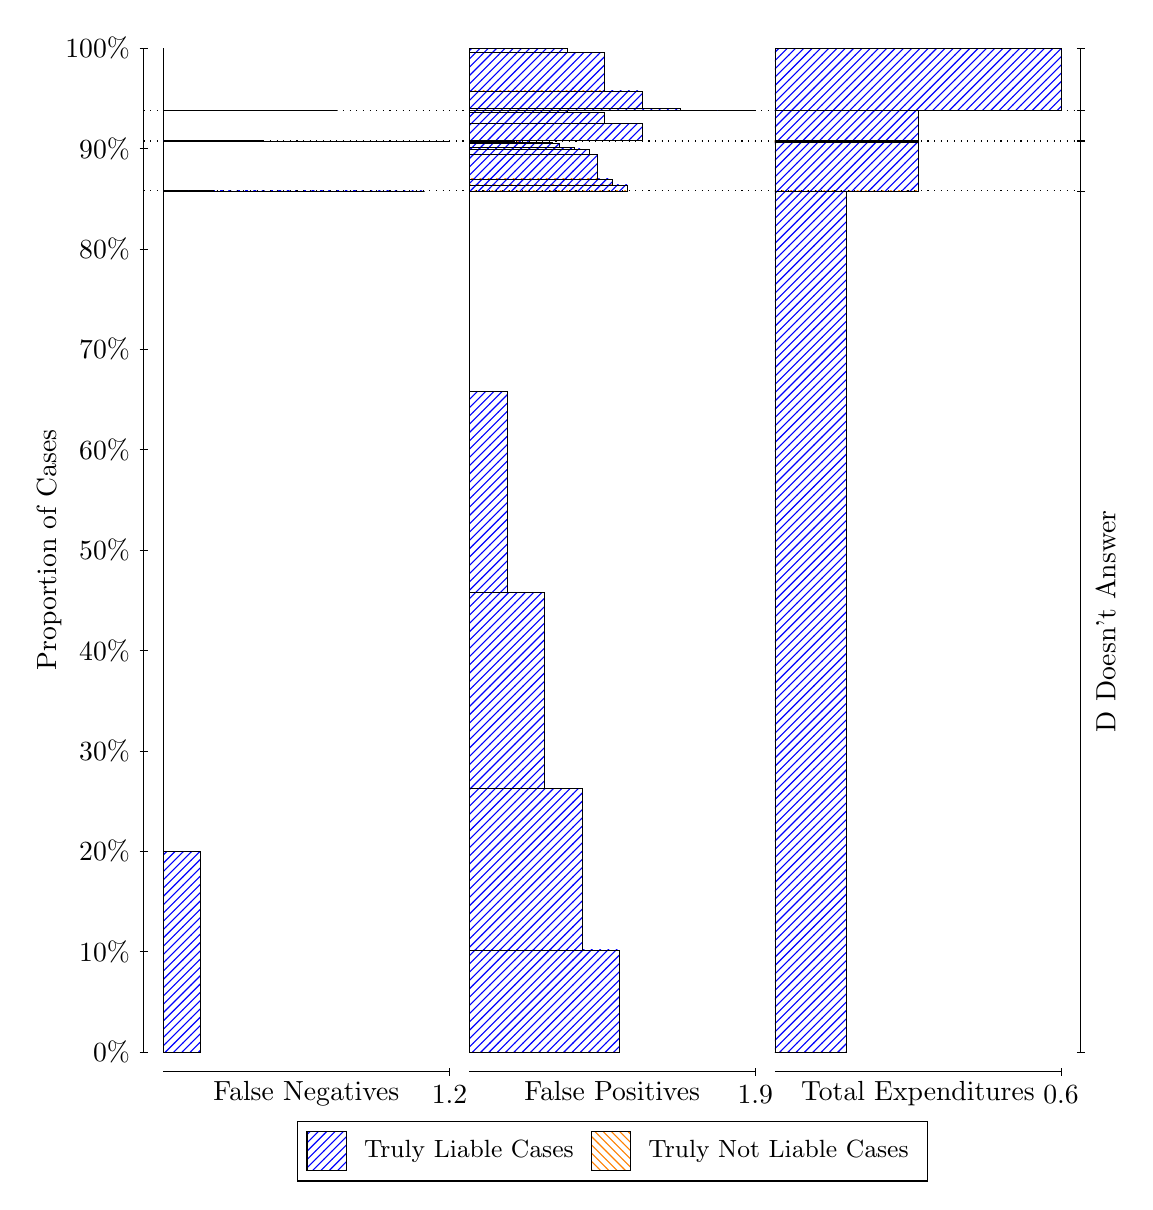
\begin{tikzpicture}
\draw[black, very thin] (1.5,1.75) -- (1.5,14.5);
\node[rotate=90, anchor=center] at (0.3, 8.125) {Proportion of Cases};
\draw[black, very thin] (1.45,1.75) -- (1.55,1.75);
\node[anchor=east] at (1.45, 1.75) {0\%};
\draw[black, very thin] (1.45,3.025) -- (1.55,3.025);
\node[anchor=east] at (1.45, 3.025) {10\%};
\draw[black, very thin] (1.45,4.3) -- (1.55,4.3);
\node[anchor=east] at (1.45, 4.3) {20\%};
\draw[black, very thin] (1.45,5.575) -- (1.55,5.575);
\node[anchor=east] at (1.45, 5.575) {30\%};
\draw[black, very thin] (1.45,6.85) -- (1.55,6.85);
\node[anchor=east] at (1.45, 6.85) {40\%};
\draw[black, very thin] (1.45,8.125) -- (1.55,8.125);
\node[anchor=east] at (1.45, 8.125) {50\%};
\draw[black, very thin] (1.45,9.4) -- (1.55,9.4);
\node[anchor=east] at (1.45, 9.4) {60\%};
\draw[black, very thin] (1.45,10.675) -- (1.55,10.675);
\node[anchor=east] at (1.45, 10.675) {70\%};
\draw[black, very thin] (1.45,11.95) -- (1.55,11.95);
\node[anchor=east] at (1.45, 11.95) {80\%};
\draw[black, very thin] (1.45,13.225) -- (1.55,13.225);
\node[anchor=east] at (1.45, 13.225) {90\%};
\draw[black, very thin] (1.45,14.5) -- (1.55,14.5);
\node[anchor=east] at (1.45, 14.5) {100\%};

\draw[black, very thin] (13.4,1.75) -- (13.4,14.5);
\draw[black, very thin] (13.35,1.75) -- (13.45,1.75);
\node[anchor=west] at (13.35, 1.75) {};
\draw[black, very thin] (13.35,12.686) -- (13.45,12.686);
\node[anchor=west] at (13.35, 12.686) {};
\draw[black, very thin] (13.35,13.315) -- (13.45,13.315);
\node[anchor=west] at (13.35, 13.315) {};
\draw[black, very thin] (13.35,13.329) -- (13.45,13.329);
\node[anchor=west] at (13.35, 13.329) {};
\draw[black, very thin] (13.35,13.708) -- (13.45,13.708);
\node[anchor=west] at (13.35, 13.708) {};
\draw[black, very thin] (13.35,14.5) -- (13.45,14.5);
\node[anchor=west] at (13.35, 14.5) {};

\draw[black, very thin, pattern color=blue, pattern=north east lines] (1.75,1.75) rectangle (2.2239,4.2999);
\draw[black, very thin, pattern color=orange, pattern=north west lines] (1.75,4.2999) rectangle (1.75,4.2999);
\draw[black, very thin, pattern color=blue, pattern=north east lines] (1.75,4.2999) rectangle (1.75,12.686);
\draw[black, very thin, pattern color=blue, pattern=north east lines] (1.75,12.686) rectangle (5.0674,12.686);
\draw[black, very thin, pattern color=blue, pattern=north east lines] (1.75,12.686) rectangle (4.7514,12.686);
\draw[black, very thin, pattern color=blue, pattern=north east lines] (1.75,12.686) rectangle (4.4355,12.686);
\draw[black, very thin, pattern color=blue, pattern=north east lines] (1.75,12.686) rectangle (4.2775,12.686);
\draw[black, very thin, pattern color=blue, pattern=north east lines] (1.75,12.686) rectangle (4.1196,12.686);
\draw[black, very thin, pattern color=blue, pattern=north east lines] (1.75,12.686) rectangle (3.9616,12.686);
\draw[black, very thin, pattern color=blue, pattern=north east lines] (1.75,12.686) rectangle (3.8036,12.686);
\draw[black, very thin, pattern color=blue, pattern=north east lines] (1.75,12.686) rectangle (3.6457,12.686);
\draw[black, very thin, pattern color=blue, pattern=north east lines] (1.75,12.686) rectangle (3.4877,12.686);
\draw[black, very thin, pattern color=blue, pattern=north east lines] (1.75,12.686) rectangle (3.3297,12.686);
\draw[black, very thin, pattern color=blue, pattern=north east lines] (1.75,12.686) rectangle (3.1717,12.686);
\draw[black, very thin, pattern color=blue, pattern=north east lines] (1.75,12.686) rectangle (3.1717,12.686);
\draw[black, very thin, pattern color=blue, pattern=north east lines] (1.75,12.686) rectangle (3.0138,12.686);
\draw[black, very thin, pattern color=blue, pattern=north east lines] (1.75,12.686) rectangle (2.8558,12.686);
\draw[black, very thin, pattern color=blue, pattern=north east lines] (1.75,12.686) rectangle (2.6978,12.686);
\draw[black, very thin, pattern color=blue, pattern=north east lines] (1.75,12.686) rectangle (2.6978,12.687);
\draw[black, very thin, pattern color=blue, pattern=north east lines] (1.75,12.687) rectangle (2.5399,12.687);
\draw[black, very thin, pattern color=blue, pattern=north east lines] (1.75,12.687) rectangle (2.3819,12.687);
\draw[black, very thin, pattern color=blue, pattern=north east lines] (1.75,12.687) rectangle (2.3819,12.688);
\draw[black, very thin, pattern color=blue, pattern=north east lines] (1.75,12.688) rectangle (2.2239,12.688);
\draw[black, very thin, pattern color=blue, pattern=north east lines] (1.75,12.688) rectangle (2.0659,12.689);
\draw[black, very thin, pattern color=blue, pattern=north east lines] (1.75,12.689) rectangle (2.0659,12.689);
\draw[black, very thin, pattern color=blue, pattern=north east lines] (1.75,12.689) rectangle (1.908,12.689);
\draw[black, very thin, pattern color=blue, pattern=north east lines] (1.75,12.689) rectangle (1.908,12.69);
\draw[black, very thin, pattern color=blue, pattern=north east lines] (1.75,12.69) rectangle (1.75,12.691);
\draw[black, very thin, pattern color=orange, pattern=north west lines] (1.75,12.691) rectangle (1.75,12.691);
\draw[black, very thin, pattern color=blue, pattern=north east lines] (1.75,12.691) rectangle (1.75,13.315);
\draw[black, very thin, pattern color=blue, pattern=north east lines] (1.75,13.315) rectangle (5.3833,13.315);
\draw[black, very thin, pattern color=blue, pattern=north east lines] (1.75,13.315) rectangle (4.5935,13.315);
\draw[black, very thin, pattern color=blue, pattern=north east lines] (1.75,13.315) rectangle (3.8036,13.315);
\draw[black, very thin, pattern color=blue, pattern=north east lines] (1.75,13.315) rectangle (3.0138,13.324);
\draw[black, very thin, pattern color=blue, pattern=north east lines] (1.75,13.324) rectangle (2.2239,13.329);
\draw[black, very thin, pattern color=orange, pattern=north west lines] (1.75,13.329) rectangle (1.75,13.329);
\draw[black, very thin, pattern color=blue, pattern=north east lines] (1.75,13.329) rectangle (2.2239,13.329);
\draw[black, very thin, pattern color=orange, pattern=north west lines] (1.75,13.329) rectangle (1.75,13.329);
\draw[black, very thin, pattern color=blue, pattern=north east lines] (1.75,13.329) rectangle (1.75,13.708);
\draw[black, very thin, pattern color=blue, pattern=north east lines] (1.75,13.708) rectangle (3.9616,13.708);
\draw[black, very thin, pattern color=blue, pattern=north east lines] (1.75,13.708) rectangle (3.1717,13.708);
\draw[black, very thin, pattern color=blue, pattern=north east lines] (1.75,13.708) rectangle (3.1717,13.708);
\draw[black, very thin, pattern color=blue, pattern=north east lines] (1.75,13.708) rectangle (2.3819,13.708);
\draw[black, very thin, pattern color=blue, pattern=north east lines] (1.75,13.708) rectangle (2.3819,13.708);
\draw[black, very thin, pattern color=orange, pattern=north west lines] (1.75,13.708) rectangle (1.75,13.708);
\draw[black, very thin, pattern color=blue, pattern=north east lines] (1.75,13.708) rectangle (1.75,14.5);
\draw[black, very thin, pattern color=orange, pattern=north west lines] (5.6333,1.75) rectangle (7.5456,1.75);
\draw[black, very thin, pattern color=blue, pattern=north east lines] (5.6333,1.75) rectangle (7.5456,3.0463);
\draw[black, very thin, pattern color=blue, pattern=north east lines] (5.6333,3.0463) rectangle (7.0675,5.1002);
\draw[black, very thin, pattern color=blue, pattern=north east lines] (5.6333,5.1002) rectangle (6.5895,7.5869);
\draw[black, very thin, pattern color=blue, pattern=north east lines] (5.6333,7.5869) rectangle (6.1114,10.136);
\draw[black, very thin, pattern color=blue, pattern=north east lines] (5.6333,10.136) rectangle (5.6333,12.686);
\draw[black, very thin, pattern color=orange, pattern=north west lines] (5.6333,12.686) rectangle (7.6412,12.686);
\draw[black, very thin, pattern color=blue, pattern=north east lines] (5.6333,12.686) rectangle (7.6412,12.761);
\draw[black, very thin, pattern color=orange, pattern=north west lines] (5.6333,12.761) rectangle (7.45,12.761);
\draw[black, very thin, pattern color=blue, pattern=north east lines] (5.6333,12.761) rectangle (7.45,12.838);
\draw[black, very thin, pattern color=orange, pattern=north west lines] (5.6333,12.838) rectangle (7.2588,12.838);
\draw[black, very thin, pattern color=blue, pattern=north east lines] (5.6333,12.838) rectangle (7.2588,13.147);
\draw[black, very thin, pattern color=blue, pattern=north east lines] (5.6333,13.147) rectangle (7.1632,13.216);
\draw[black, very thin, pattern color=orange, pattern=north west lines] (5.6333,13.216) rectangle (7.0675,13.216);
\draw[black, very thin, pattern color=blue, pattern=north east lines] (5.6333,13.216) rectangle (7.0675,13.218);
\draw[black, very thin, pattern color=blue, pattern=north east lines] (5.6333,13.218) rectangle (6.9719,13.24);
\draw[black, very thin, pattern color=orange, pattern=north west lines] (5.6333,13.24) rectangle (6.8763,13.24);
\draw[black, very thin, pattern color=blue, pattern=north east lines] (5.6333,13.24) rectangle (6.8763,13.242);
\draw[black, very thin, pattern color=blue, pattern=north east lines] (5.6333,13.242) rectangle (6.7807,13.285);
\draw[black, very thin, pattern color=orange, pattern=north west lines] (5.6333,13.285) rectangle (6.6851,13.285);
\draw[black, very thin, pattern color=blue, pattern=north east lines] (5.6333,13.285) rectangle (6.6851,13.3);
\draw[black, very thin, pattern color=orange, pattern=north west lines] (5.6333,13.3) rectangle (6.6851,13.3);
\draw[black, very thin, pattern color=blue, pattern=north east lines] (5.6333,13.3) rectangle (6.6851,13.302);
\draw[black, very thin, pattern color=blue, pattern=north east lines] (5.6333,13.302) rectangle (6.5895,13.304);
\draw[black, very thin, pattern color=blue, pattern=north east lines] (5.6333,13.304) rectangle (6.4939,13.305);
\draw[black, very thin, pattern color=orange, pattern=north west lines] (5.6333,13.305) rectangle (6.4939,13.305);
\draw[black, very thin, pattern color=blue, pattern=north east lines] (5.6333,13.305) rectangle (6.4939,13.306);
\draw[black, very thin, pattern color=blue, pattern=north east lines] (5.6333,13.306) rectangle (6.3982,13.309);
\draw[black, very thin, pattern color=orange, pattern=north west lines] (5.6333,13.309) rectangle (6.3026,13.309);
\draw[black, very thin, pattern color=blue, pattern=north east lines] (5.6333,13.309) rectangle (6.3026,13.309);
\draw[black, very thin, pattern color=blue, pattern=north east lines] (5.6333,13.309) rectangle (6.207,13.31);
\draw[black, very thin, pattern color=blue, pattern=north east lines] (5.6333,13.31) rectangle (6.207,13.312);
\draw[black, very thin, pattern color=orange, pattern=north west lines] (5.6333,13.312) rectangle (6.1114,13.312);
\draw[black, very thin, pattern color=blue, pattern=north east lines] (5.6333,13.312) rectangle (6.1114,13.312);
\draw[black, very thin, pattern color=blue, pattern=north east lines] (5.6333,13.312) rectangle (6.0158,13.312);
\draw[black, very thin, pattern color=blue, pattern=north east lines] (5.6333,13.312) rectangle (6.0158,13.314);
\draw[black, very thin, pattern color=blue, pattern=north east lines] (5.6333,13.314) rectangle (5.9202,13.314);
\draw[black, very thin, pattern color=blue, pattern=north east lines] (5.6333,13.314) rectangle (5.8246,13.315);
\draw[black, very thin, pattern color=blue, pattern=north east lines] (5.6333,13.315) rectangle (5.7289,13.315);
\draw[black, very thin, pattern color=blue, pattern=north east lines] (5.6333,13.315) rectangle (5.7289,13.315);
\draw[black, very thin, pattern color=blue, pattern=north east lines] (5.6333,13.315) rectangle (5.6333,13.315);
\draw[black, very thin, pattern color=orange, pattern=north west lines] (5.6333,13.315) rectangle (5.9202,13.315);
\draw[black, very thin, pattern color=blue, pattern=north east lines] (5.6333,13.315) rectangle (5.9202,13.321);
\draw[black, very thin, pattern color=blue, pattern=north east lines] (5.6333,13.321) rectangle (5.6333,13.329);
\draw[black, very thin, pattern color=orange, pattern=north west lines] (5.6333,13.329) rectangle (7.8325,13.329);
\draw[black, very thin, pattern color=blue, pattern=north east lines] (5.6333,13.329) rectangle (7.8325,13.547);
\draw[black, very thin, pattern color=blue, pattern=north east lines] (5.6333,13.547) rectangle (7.3544,13.682);
\draw[black, very thin, pattern color=blue, pattern=north east lines] (5.6333,13.682) rectangle (6.8763,13.707);
\draw[black, very thin, pattern color=blue, pattern=north east lines] (5.6333,13.707) rectangle (6.3982,13.708);
\draw[black, very thin, pattern color=blue, pattern=north east lines] (5.6333,13.708) rectangle (5.9202,13.708);
\draw[black, very thin, pattern color=orange, pattern=north west lines] (5.6333,13.708) rectangle (9.2667,13.708);
\draw[black, very thin, pattern color=blue, pattern=north east lines] (5.6333,13.708) rectangle (9.2667,13.708);
\draw[black, very thin, pattern color=orange, pattern=north west lines] (5.6333,13.708) rectangle (8.7886,13.708);
\draw[black, very thin, pattern color=blue, pattern=north east lines] (5.6333,13.708) rectangle (8.7886,13.708);
\draw[black, very thin, pattern color=orange, pattern=north west lines] (5.6333,13.708) rectangle (8.3105,13.708);
\draw[black, very thin, pattern color=blue, pattern=north east lines] (5.6333,13.708) rectangle (8.3105,13.73);
\draw[black, very thin, pattern color=orange, pattern=north west lines] (5.6333,13.73) rectangle (7.8325,13.73);
\draw[black, very thin, pattern color=blue, pattern=north east lines] (5.6333,13.73) rectangle (7.8325,13.957);
\draw[black, very thin, pattern color=orange, pattern=north west lines] (5.6333,13.957) rectangle (7.3544,13.957);
\draw[black, very thin, pattern color=blue, pattern=north east lines] (5.6333,13.957) rectangle (7.3544,14.445);
\draw[black, very thin, pattern color=blue, pattern=north east lines] (5.6333,14.445) rectangle (6.8763,14.5);
\draw[black, very thin, pattern color=blue, pattern=north east lines] (5.6333,14.5) rectangle (6.3982,14.5);
\draw[black, very thin, pattern color=blue, pattern=north east lines] (5.6333,14.5) rectangle (5.9202,14.5);
\draw[black, very thin, pattern color=blue, pattern=north east lines] (5.6333,14.5) rectangle (5.6333,14.5);
\draw[black, very thin, pattern color=orange, pattern=north west lines] (9.5167,1.75) rectangle (10.425,1.75);
\draw[black, very thin, pattern color=blue, pattern=north east lines] (9.5167,1.75) rectangle (10.425,12.686);
\draw[black, very thin, pattern color=orange, pattern=north west lines] (9.5167,12.686) rectangle (11.333,12.686);
\draw[black, very thin, pattern color=blue, pattern=north east lines] (9.5167,12.686) rectangle (11.333,13.308);
\draw[black, very thin, pattern color=orange, pattern=north west lines] (9.5167,13.308) rectangle (11.333,13.308);
\draw[black, very thin, pattern color=blue, pattern=north east lines] (9.5167,13.308) rectangle (11.333,13.309);
\draw[black, very thin, pattern color=orange, pattern=north west lines] (9.5167,13.309) rectangle (11.333,13.309);
\draw[black, very thin, pattern color=blue, pattern=north east lines] (9.5167,13.309) rectangle (11.333,13.315);
\draw[black, very thin, pattern color=orange, pattern=north west lines] (9.5167,13.315) rectangle (11.333,13.315);
\draw[black, very thin, pattern color=blue, pattern=north east lines] (9.5167,13.315) rectangle (11.333,13.329);
\draw[black, very thin, pattern color=orange, pattern=north west lines] (9.5167,13.329) rectangle (11.333,13.329);
\draw[black, very thin, pattern color=blue, pattern=north east lines] (9.5167,13.329) rectangle (11.333,13.708);
\draw[black, very thin, pattern color=orange, pattern=north west lines] (9.5167,13.708) rectangle (13.15,13.708);
\draw[black, very thin, pattern color=blue, pattern=north east lines] (9.5167,13.708) rectangle (13.15,14.5);
\draw[black, dotted] (1.5,12.686) -- (13.4,12.686);
\draw[black, dotted] (1.5,13.315) -- (13.4,13.315);
\draw[black, dotted] (1.5,13.329) -- (13.4,13.329);
\draw[black, dotted] (1.5,13.708) -- (13.4,13.708);
\draw[black, very thin] (1.75,1.5) -- (5.3833,1.5);
\node[anchor=north] at (3.5667, 1.5) {False Negatives};
\draw[black, very thin] (5.3833,1.45) -- (5.3833,1.55);
\node[anchor=north] at (5.3833, 1.45) {1.2};

\draw[black, very thin] (5.6333,1.5) -- (9.2667,1.5);
\node[anchor=north] at (7.45, 1.5) {False Positives};
\draw[black, very thin] (9.2667,1.45) -- (9.2667,1.55);
\node[anchor=north] at (9.2667, 1.45) {1.9};

\draw[black, very thin] (9.5167,1.5) -- (13.15,1.5);
\node[anchor=north] at (11.333, 1.5) {Total Expenditures};
\draw[black, very thin] (13.15,1.45) -- (13.15,1.55);
\node[anchor=north] at (13.15, 1.45) {0.6};

\node[black, centered, rotate=90] at (13.72, 7.2182) {D Doesn't Answer};





\draw (7.449999999999999,1.5) node[draw=none] (baseCoordinate) {};
\begin{scope}[align=center]
        \matrix[scale=0.5, draw=black, below=0.5cm of baseCoordinate, nodes={draw}, column sep=0.1cm]{
            \node[rectangle, draw, minimum width=0.5cm, minimum height=0.5cm, pattern=north east lines, pattern color=blue] {}; &
            \node[draw=none, font=\small] (B) {Truly Liable Cases}; &
            \node[rectangle, draw, minimum width=0.5cm, minimum height=0.5cm, pattern=north west lines, pattern color=orange] {}; &
            \node[draw=none, font=\small] (B) {Truly Not Liable Cases}; \\
            };
\end{scope}

\end{tikzpicture}
\end{document}